\documentclass[12pt, a4paper]{article}

\usepackage[utf8]{inputenc}
\usepackage[T1]{fontenc}
\usepackage[margin=2.5cm]{geometry}
\usepackage{hyperref}
\usepackage{listings}
\usepackage{xcolor}
\usepackage{booktabs}
\usepackage{array}
\usepackage{enumitem}
\usepackage{titlesec}
\usepackage{fancyhdr}
\usepackage{amsmath}
\usepackage{tikz}
\usetikzlibrary{shapes.geometric, arrows.meta, positioning, fit, backgrounds}

% ── Colors ──────────────────────────────────────────────────────────────────
\definecolor{dxcpurple}{RGB}{102, 0, 153}
\definecolor{codebg}{RGB}{245, 245, 245}
\definecolor{codeframe}{RGB}{200, 200, 200}
\definecolor{keywordcolor}{RGB}{0, 0, 180}
\definecolor{stringcolor}{RGB}{163, 21, 21}
\definecolor{commentcolor}{RGB}{0, 128, 0}
\definecolor{boxgreen}{RGB}{220, 240, 220}
\definecolor{boxorange}{RGB}{255, 235, 210}
\definecolor{boxred}{RGB}{255, 215, 215}

% ── Code style ──────────────────────────────────────────────────────────────
\lstdefinestyle{python}{
    language=Python,
    backgroundcolor=\color{codebg},
    frame=single,
    rulecolor=\color{codeframe},
    basicstyle=\ttfamily\small,
    keywordstyle=\color{keywordcolor}\bfseries,
    stringstyle=\color{stringcolor},
    commentstyle=\color{commentcolor}\itshape,
    numbers=left,
    numberstyle=\tiny\color{gray},
    numbersep=8pt,
    breaklines=true,
    breakatwhitespace=true,
    tabsize=4,
    showstringspaces=false,
    captionpos=b,
}

% ── Header / Footer ─────────────────────────────────────────────────────────
\pagestyle{fancy}
\fancyhf{}
\fancyhead[L]{\textcolor{dxcpurple}{\textbf{DXC Technology}}}
\fancyhead[R]{\textcolor{dxcpurple}{Name Matching Algorithm}}
\fancyfoot[C]{\thepage}
\renewcommand{\headrulewidth}{0.4pt}
\renewcommand{\headrule}{\hbox to\headwidth{\color{dxcpurple}\leaders\hrule height \headrulewidth\hfill}}

% ── Section colors ───────────────────────────────────────────────────────────
\titleformat{\section}{\large\bfseries\color{dxcpurple}}{}{0em}{}[\titlerule]
\titleformat{\subsection}{\normalsize\bfseries\color{dxcpurple}}{}{0em}{}

% ── Hyperref ────────────────────────────────────────────────────────────────
\hypersetup{
    colorlinks=true,
    linkcolor=dxcpurple,
    urlcolor=dxcpurple,
}

% ────────────────────────────────────────────────────────────────────────────
\begin{document}

% ── Title page ──────────────────────────────────────────────────────────────
\begin{titlepage}
    \centering
    \vspace*{2cm}
    {\color{dxcpurple}\rule{\linewidth}{1.5pt}}\\[0.5cm]
    {\Huge\bfseries\color{dxcpurple} Person Name Matching}\\[0.3cm]
    {\Large Technical Design Document}\\[0.3cm]
    {\color{dxcpurple}\rule{\linewidth}{1.5pt}}\\[2cm]

    {\large\textbf{Project:} IRP AUTO — DXC GraphTalk Service Desk Reporting System}\\[0.5cm]
    {\large\textbf{Component:} Team Tab — Availability $\leftrightarrow$ Jira Assignee Reconciliation}\\[2cm]

    \begin{tabular}{ll}
        \textbf{Author}  & El Adnani Ali \\[0.3cm]
        \textbf{Date}    & April 2, 2026 \\[0.3cm]
        \textbf{Version} & 1.0 \\[0.3cm]
        \textbf{Status}  & Production \\
    \end{tabular}

    \vfill
    {\color{dxcpurple}\rule{\linewidth}{0.4pt}}\\[0.2cm]
    {\small DXC Technology — IRP AUTO Service Desk Analytics Platform}
\end{titlepage}

\tableofcontents
\newpage

% ────────────────────────────────────────────────────────────────────────────
\section{Problem Statement}

The reporting dashboard draws data from two independent sources that refer to the same
people using inconsistent name formats:

\begin{itemize}
    \item \textbf{Team Availability Sheet} (Release Lifecycle Excel file) — names entered
          manually by the project manager. Examples: \texttt{GHAOUTI, SOUFIANE},
          \texttt{Mohamed jaouad}, \texttt{sara ghaoui}.

    \item \textbf{Jira Assignee Field} — the \texttt{displayName} from each user's
          Atlassian account profile. Examples: \texttt{GHAOUTI, SOUFIANE},
          \texttt{Mohamed Jaouad}, \texttt{Sara Ghaoui}.
\end{itemize}

To compute team productivity metrics (SP delivered per person, capacity vs.\ output, squad
breakdown), the system must \textbf{link each availability-sheet person to their
corresponding Jira tickets}. This linkage cannot be done with a simple equality check
because:

\begin{itemize}
    \item Capitalisation varies (\texttt{sara ghaoui} vs.\ \texttt{Sara Ghaoui}).
    \item First and last name order may differ (\texttt{GHAOUTI, SOUFIANE} vs.\
          \texttt{Soufiane Ghaouti}).
    \item Diacritics may be dropped (\texttt{Benali} vs.\ \texttt{Bénali}).
    \item Spelling variants exist in practice (\texttt{hamyouni} vs.\ \texttt{hamyoumi}).
    \item Some people appear under their email prefix in one system.
    \item Common first names like \textit{Mohamed} / \textit{Mohammed} are shared by
          multiple team members, making first-name-only matches unreliable.
\end{itemize}

A \textbf{fuzzy name matching} algorithm was designed and implemented in Python to solve
this problem robustly.

% ────────────────────────────────────────────────────────────────────────────
\section{Algorithm Overview}

The matching process runs in three stages:

\begin{enumerate}
    \item \textbf{Normalisation} — both names are cleaned and reduced to a canonical,
          order-independent token set.
    \item \textbf{Scoring} — a similarity score between 0 and 1 is computed for every
          (Jira name, availability name) pair.
    \item \textbf{Greedy exclusive assignment} — pairs are sorted by score descending and
          assigned one-to-one, so each Jira assignee maps to at most one availability
          person and vice versa.
\end{enumerate}

\vspace{0.8cm}

% ── Flow diagram ────────────────────────────────────────────────────────────
\begin{center}
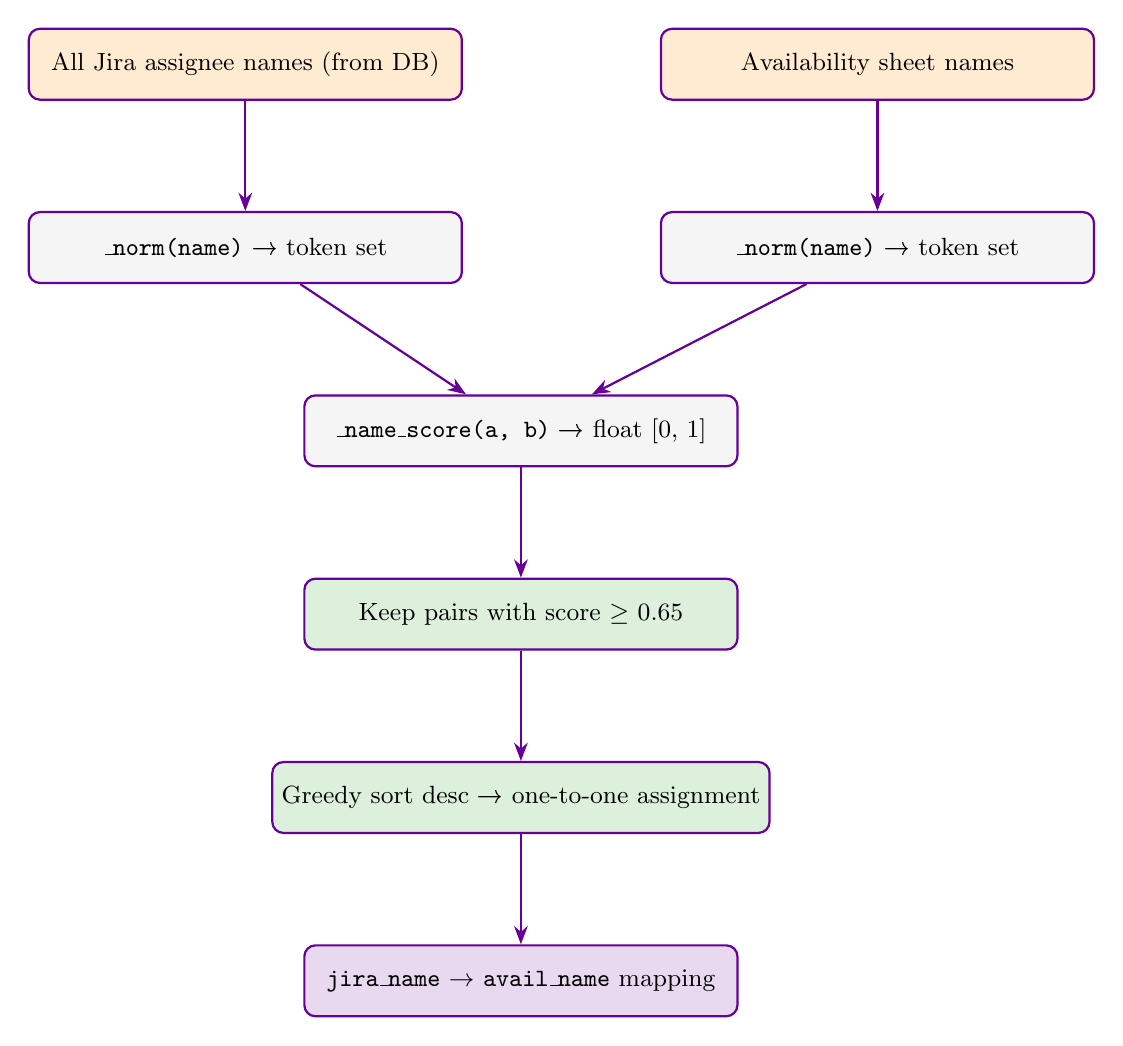
\begin{tikzpicture}[
    node distance=1.4cm,
    box/.style={rectangle, draw=dxcpurple, thick, rounded corners=4pt,
                minimum width=5.5cm, minimum height=0.9cm,
                text centered, font=\small},
    arrow/.style={-Stealth, thick, color=dxcpurple},
]
    \node[box, fill=boxorange] (A) {All Jira assignee names (from DB)};
    \node[box, fill=boxorange, right=2.5cm of A] (B) {Availability sheet names};
    \node[box, fill=codebg, below=of A] (normA) {\texttt{\_norm(name)} → token set};
    \node[box, fill=codebg, below=of B] (normB) {\texttt{\_norm(name)} → token set};
    \node[box, fill=codebg, below=1.4cm of normA, xshift=3.5cm] (score)
          {\texttt{\_name\_score(a, b)} → float [0, 1]};
    \node[box, fill=boxgreen, below=1.4cm of score] (filter)
          {Keep pairs with score $\geq$ 0.65};
    \node[box, fill=boxgreen, below=1.4cm of filter] (greedy)
          {Greedy sort desc → one-to-one assignment};
    \node[box, fill=dxcpurple!15, below=1.4cm of greedy] (out)
          {\texttt{jira\_name} $\to$ \texttt{avail\_name} mapping};

    \draw[arrow] (A) -- (normA);
    \draw[arrow] (B) -- (normB);
    \draw[arrow] (normA) -- (score);
    \draw[arrow] (normB) -- (score);
    \draw[arrow] (score) -- (filter);
    \draw[arrow] (filter) -- (greedy);
    \draw[arrow] (greedy) -- (out);
\end{tikzpicture}
\end{center}

% ────────────────────────────────────────────────────────────────────────────
\section{Step 1 — Name Normalisation}

\subsection{Purpose}

Normalisation removes superficial formatting differences so that
\texttt{GHAOUTI, SOUFIANE}, \texttt{soufiane ghaouti}, and \texttt{Ghaouti Soufiane}
all become the same canonical form before any comparison takes place.

\subsection{Implementation}

\begin{lstlisting}[style=python, caption={\_norm: canonical token set}]
import re

def _norm(s: str) -> str:
    """Normalize a person name for fuzzy matching."""
    s = str(s).lower()

    # If it looks like an email, keep only the local part (before @)
    if "@" in s:
        s = s.split("@")[0]

    # Remove parenthetical qualifiers: (BA), (SAAS_FR), etc.
    s = re.sub(r"\(.*?\)", "", s)

    # Replace punctuation with spaces: commas, dots, dashes, underscores
    s = re.sub(r"[,\.\-_@]", " ", s)

    # Collapse multiple whitespace into one
    s = re.sub(r"\s+", " ", s).strip()

    # Sort tokens alphabetically so name order never matters
    # Drop single-character tokens (initials like "J." after cleanup)
    tokens = sorted(t for t in s.split() if len(t) > 1)

    return " ".join(tokens)
\end{lstlisting}

\subsection{Transformation Examples}

\begin{center}
\begin{tabular}{>{\ttfamily}l >{\ttfamily}l}
    \toprule
    \normalfont\textbf{Raw input} & \normalfont\textbf{After \_norm()} \\
    \midrule
    GHAOUTI, SOUFIANE            & ghaouti soufiane \\
    Soufiane Ghaouti             & ghaouti soufiane \\
    Mohamed jaouad               & jaouad mohamed \\
    Mohamed Jaouad               & jaouad mohamed \\
    ali.eladnani@dxc.com         & ali eladnani \\
    sara ghaoui (BA)             & ghaoui sara \\
    BENMANSOUR MEHDI             & benmansour mehdi \\
    Mehdi Benmansour             & benmansour mehdi \\
    hamyouni                     & hamyouni \\
    hamyoumi                     & hamyoumi \\
    \bottomrule
\end{tabular}
\end{center}

\noindent
Note that token sorting makes \texttt{GHAOUTI, SOUFIANE} and \texttt{Soufiane Ghaouti}
produce \textbf{identical} normalised strings, even though the original order is reversed.

% ────────────────────────────────────────────────────────────────────────────
\section{Step 2 — Similarity Scoring}

\subsection{Design Rationale}

A straightforward approach would be to compare the full normalised strings using a standard
string similarity metric like Levenshtein distance or \texttt{SequenceMatcher}. However,
this breaks down for names like \texttt{Mohamed} / \texttt{Mohammed} — these are nearly
identical strings but belong to different people on the same team. A full-string approach
would incorrectly merge them.

The chosen approach is \textbf{per-token matching}: split both names into individual words
and check how many words from the shorter name find a match in the longer name. This
requires \textit{at least two tokens to agree} (typically first name + last name) before
a pair is considered a match, making it robust against common-first-name collisions.

\subsection{Implementation}

\begin{lstlisting}[style=python, caption={\_name\_score: per-token similarity}]
import difflib

def _name_score(a: str, b: str) -> float:
    """
    Per-token matching score between two person names.

    For each token in the shorter name, find its best-matching token
    in the longer name:
      - Exact match           -> +1.0
      - Near-identical match  -> +0.8  (SequenceMatcher ratio >= 0.85)
      - No match              -> +0.0

    Score = total_matched / len(shorter_name_tokens)
    Range: [0.0, 1.0]
    """
    na, nb = _norm(a), _norm(b)
    ta = list(set(na.split()))   # deduplicate tokens
    tb = list(set(nb.split()))

    if not ta or not tb:
        return 0.0

    # Always iterate over the shorter token list
    shorter, longer = (ta, tb) if len(ta) <= len(tb) else (tb, ta)
    longer_set = set(longer)

    matched = 0.0
    for token in shorter:
        if token in longer_set:
            matched += 1.0          # exact token match
        else:
            best_ratio = max(
                difflib.SequenceMatcher(None, token, u).ratio()
                for u in longer
            )
            if best_ratio >= 0.85:
                matched += 0.8      # partial credit for near-identical spelling

    return matched / len(shorter)
\end{lstlisting}

\subsection{Scoring Examples}

\begin{center}
\begin{tabular}{llc}
    \toprule
    \textbf{Name A} & \textbf{Name B} & \textbf{Score} \\
    \midrule
    GHAOUTI, SOUFIANE   & Soufiane Ghaouti  & 1.00 \\
    Mohamed jaouad      & Mohamed Jaouad    & 1.00 \\
    BENMANSOUR MEHDI    & Mehdi Benmansour  & 1.00 \\
    hamyouni            & hamyoumi          & 0.80 \\
    Mohamed jaouad      & Mohamed Hamama    & 0.50 \\
    sara ghaoui         & sara ghaoui       & 1.00 \\
    Jean-Luc LERMA      & Jean Luc Lerma    & 1.00 \\
    Mohamed             & Mohammed          & 0.80 \\
    Ali                 & Alioui            & 0.00 (below 0.85 ratio) \\
    \bottomrule
\end{tabular}
\end{center}

\subsection{Why the 0.85 Fuzzy Sub-Token Threshold?}

The \texttt{SequenceMatcher} ratio for \texttt{hamyouni} vs.\ \texttt{hamyoumi} is
approximately $0.94$ — above the 0.85 threshold, so they receive partial credit of 0.8.
The ratio for clearly different tokens (e.g.\ \texttt{ghaoui} vs.\ \texttt{benali})
is typically below 0.50, well below 0.85. The 0.85 threshold was calibrated to capture
real spelling variants (typos, transliteration differences) while rejecting unrelated tokens.

% ────────────────────────────────────────────────────────────────────────────
\section{Step 3 — Greedy Exclusive Assignment}

\subsection{Purpose}

After scoring all pairs, there may be multiple availability names that score above the
threshold for the same Jira person (or vice versa). The assignment step ensures that:

\begin{itemize}
    \item Each Jira assignee is linked to \textbf{at most one} availability person.
    \item The assignment is \textbf{globally optimal} in the sense that highest-confidence
          pairs are resolved first.
\end{itemize}

\subsection{Implementation}

\begin{lstlisting}[style=python, caption={Greedy exclusive one-to-one assignment}]
# 1. Build all candidate pairs above threshold
_pair_scores = []
for _jn in _all_jira_assignees:
    for _an in _unique_avail_names:
        score = _name_score(_jn, _an)
        if score >= 0.65:
            _pair_scores.append({"jira": _jn, "avail": _an, "score": score})

# 2. Sort by score descending (best matches first)
# 3. Greedy assignment: take the best pair, mark the Jira name as used
_jira_to_avail = {}
for pair in sorted(_pair_scores, key=lambda x: -x["score"]):
    if pair["jira"] not in _jira_to_avail:
        _jira_to_avail[pair["jira"]] = pair["avail"]

# 4. Invert map: avail person -> list of their Jira names
#    (one person may appear under multiple Jira accounts)
_avail_to_jiras = {}
for jira_name, avail_name in _jira_to_avail.items():
    _avail_to_jiras.setdefault(avail_name, []).append(jira_name)
\end{lstlisting}

\subsection{Why Greedy (Not Optimal)?}

An optimal one-to-one matching would use the Hungarian algorithm ($O(n^3)$). With a team
size of approximately 20--30 people, the greedy approach (sort once, iterate) is
indistinguishable in result from the optimal solution and runs in microseconds.
The greedy method also has a practical advantage: it is trivial to understand and debug
— the highest-confidence pair is always resolved first, making the output easy to audit.

\subsection{Threshold Choice: 0.65}

The main matching threshold of \textbf{0.65} means that a Jira name is only linked to an
availability person if at least 65\% of the shorter name's tokens find a match. In practice:

\begin{itemize}
    \item A two-token name (first + last) requires \textbf{both tokens} to match at
          some level (exact or near-exact) to score $\geq$ 0.65.
    \item A single-token name (e.g.\ \texttt{ouyahia}) requires that one token to match
          exactly (score = 1.0) to pass the threshold.
    \item This eliminates false positives where only a common first name like
          \textit{Mohamed} matches.
\end{itemize}

% ────────────────────────────────────────────────────────────────────────────
\section{AQ Roster Matching (Squad Assignment)}

\subsection{Context}

The scope file (Release Lifecycle Excel) contains a secondary roster in columns AP and AQ:
a list of team members with their assigned squad. These names are used to determine which
squad each person belongs to, independently of the availability sheet.

\subsection{Lower Threshold: 0.55}

For squad assignment, the matching threshold is relaxed to \textbf{0.55}:

\begin{lstlisting}[style=python, caption={AQ roster to Jira name matching (threshold 0.55)}]
for _raw_name, _squad in _sa_squad.items():
    _best_jn, _best_score = None, 0.0
    for _jn in _matched_jira_names:
        _sc = _name_score(_raw_name, _jn)
        if _sc > _best_score:
            _best_score, _best_jn = _sc, _jn
    if _best_jn and _best_score >= 0.55:   # <-- relaxed threshold
        _jn_squad_map[_best_jn] = _squad
\end{lstlisting}

\noindent
The lower threshold is justified because:

\begin{itemize}
    \item The AQ roster is used only to assign a squad label, not to attribute productivity
          metrics. A false match here causes a wrong squad label but does not inflate or
          deflate any numeric metric.
    \item Names in the AQ roster are sometimes abbreviated or partially entered, making
          a 0.65 threshold too strict.
\end{itemize}

% ────────────────────────────────────────────────────────────────────────────
\section{Three-Level Squad Lookup}

After the name matching establishes the Jira $\to$ availability mapping, squad assignment
follows a three-level priority chain:

\begin{enumerate}
    \item \textbf{AQ roster} (columns AP/AQ of the scope file) — authoritative source.
          Every person listed there gets their squad from this table, matched via the
          0.55-threshold fuzzy match described in Section~5.

    \item \textbf{Scope ticket key $\to$ squad} — if a Jira assignee owns scope tickets,
          the squad is inferred from those ticket rows. The mode (most frequent) squad
          across all scope tickets for that person is used.

    \item \textbf{Availability sheet squad column} — fallback for anyone not found in
          levels 1 or 2. Transverse is excluded at this level (normalised to ``—'').
\end{enumerate}

\subsection{Squad Name Normalisation}

Squad names appear in different languages and spellings across the two source files
(French in the availability sheet, English in the scope file). A normalisation function
maps all variants to a canonical English label:

\begin{center}
\begin{tabular}{ll}
    \toprule
    \textbf{Raw value (any source)} & \textbf{Canonical squad name} \\
    \midrule
    Contrats \& Santé, contrat, sant\ldots    & Health \& Contracts \& Persons \\
    Health \& Contracts \& Persons            & Health \& Contracts \& Persons \\
    Editique, Éditique                        & Printing \\
    Printing                                  & Printing \\
    Comptabilité/PDM, Compta, comptab\ldots   & Accounting/PDM/BI \\
    Accounting/PDM/BI, pdm\ldots              & Accounting/PDM/BI \\
    Prévoyance, pr\ldots voyance              & Risk \& Protection \\
    Risk \& Protection                        & Risk \& Protection \\
    DSN/FLUX FINANCIER                        & DSN/FLUX FINANCIER \\
    Transverse                                & — (excluded) \\
    \bottomrule
\end{tabular}
\end{center}

% ────────────────────────────────────────────────────────────────────────────
\section{Edge Case: People Not in the Availability Sheet}

Some team members own scope tickets but do not appear in the availability sheet. The
canonical example is \textbf{Jean-Luc LERMA} (squad TMA), who has scope ticket
\texttt{IRPAUTO-16997} but is absent from the availability sheet.

Such people would be silently excluded from the team charts because:
\begin{itemize}
    \item They fail the 0.65 threshold against all availability names (no match found).
    \item \texttt{\_matched\_jira\_names} does not include them.
    \item The squad chart pool only draws from \texttt{\_matched\_jira\_names}.
\end{itemize}

\textbf{Solution — supplementary scope-extra lookup:}

\begin{lstlisting}[style=python, caption={Supplementary lookup for non-availability scope owners}]
_scope_extra_jn_squad = {}

_scope_ticket_assignees = (
    _df_all[_df_all["key"].isin(scope_keys)]
    ["assignee"].dropna().unique()
)

for _jn in _scope_ticket_assignees:
    # Skip people already matched through the normal path
    if _jn in _matched_jira_names or _jn in _jn_squad_map:
        continue
    # Find the squad from whichever scope ticket they own
    for _k in _df_all[_df_all["assignee"] == _jn]["key"]:
        if _k in _scope_key_squad:
            _scope_extra_jn_squad[_jn] = _scope_key_squad[_k]
            break

# Extend the squad chart pool to include these extra assignees
_all_squad_chart_jn = _matched_jira_names | set(_scope_extra_jn_squad.keys())

# Merge both maps, _jn_squad_map takes priority
_combined_squad_map = {**_scope_extra_jn_squad, **_jn_squad_map}
\end{lstlisting}

% ────────────────────────────────────────────────────────────────────────────
\section{Summary of Parameters}

\begin{center}
\begin{tabular}{lll}
    \toprule
    \textbf{Parameter} & \textbf{Value} & \textbf{Purpose} \\
    \midrule
    Main match threshold       & 0.65 & Availability $\leftrightarrow$ Jira linkage \\
    AQ roster threshold        & 0.55 & Squad assignment from scope file roster \\
    Fuzzy sub-token threshold  & 0.85 & Partial credit for near-identical tokens \\
    Partial credit weight      & 0.80 & Score added for a fuzzy (non-exact) token match \\
    Min token length           & 2    & Single-character tokens (initials) are ignored \\
    \bottomrule
\end{tabular}
\end{center}

% ────────────────────────────────────────────────────────────────────────────
\section{Output Structures}

After the matching runs, three dictionaries drive all downstream computations in the
Team tab:

\begin{center}
\begin{tabular}{lp{9cm}}
    \toprule
    \textbf{Variable} & \textbf{Content} \\
    \midrule
    \texttt{\_jira\_to\_avail}  &
        \texttt{\{jira\_name: avail\_name\}} — one entry per matched Jira assignee. \\[0.3cm]
    \texttt{\_avail\_to\_jiras} &
        \texttt{\{avail\_name: [jira\_name, ...]\}} — inverse map; one person may appear
        under multiple Jira display names (e.g.\ different account registrations). \\[0.3cm]
    \texttt{\_matched\_jira\_names} &
        \texttt{set} of all Jira names that were successfully matched. Only these names
        are included in KPI cards and individual productivity charts. \\
    \bottomrule
\end{tabular}
\end{center}

\vspace{1cm}
\noindent\rule{\linewidth}{0.4pt}
{\small\textit{Document generated on April 2, 2026 — DXC Technology, IRP AUTO Analytics Platform.}}

\end{document}
